\subsection{SOAC: scan}

Second-order Array Combinator (SOAC):\textcolor{red}{\textit{\textbf{scan}}} 是所有的循环神经网络(recurrent neural networks)背后的核心并行pattern。接口和语义如下:

\begin{equation*}
    \begin{aligned}
        \textbf{scan} &::(\alpha, \beta \rightarrow \alpha) \rightarrow \alpha \rightarrow[\beta]^d_n \rightarrow [\alpha]_n^d \\
        \mathbf{scan} \ \oplus \ \textit{xs} &= [x_0,\ x_0 \oplus x_1, \dotsb,\ x_0 \oplus x_1 \dotsb \oplus x_n ] \\
        \mathbf{scanl} \ \oplus \ I \ \textit{xs} &= \left[
            I \oplus x_0,\  ((I \oplus x_0) \oplus x_1), \ \dotsb,
            \ (((I \oplus x_0)\oplus x_1)\dotsb \oplus x_{n-1})
        \right] \\
        \mathbf{scanr} \ \oplus \ I \ \textit{xs} &= \left[
            (x_0 \oplus (x_{n-2} \oplus (x_{n-1} \oplus I)))
            ,\ \dotsb, \ (x_{n-2} \oplus (x_{n-1} \oplus I)),
            \ x_{n-1} \oplus I \right] \\
    \end{aligned}
\end{equation*}


% If $\oplus$ is associative, scan can be executed in parallel\cite{DBLP:journals/tc/Blelloch89}.
% If $\oplus$ is left associative, scanl is used. If $\oplus$ is right associative, scanr is used. The first operand of $\oplus$ carries a data dependence with a distance of 1\cite{DBLP:journals/tpds/WolfL91}.

% \subsection{RNN}

% As shown in Figure \ref{scan-step}, in one computational step, a cell processing unit $\otimes$ produces a new token $y$ by aggregating a token $x$ from a token stream $xs$ with another token $y'$ created in the previous computational step.

% \begin{figure}[h]
%     \centering
%     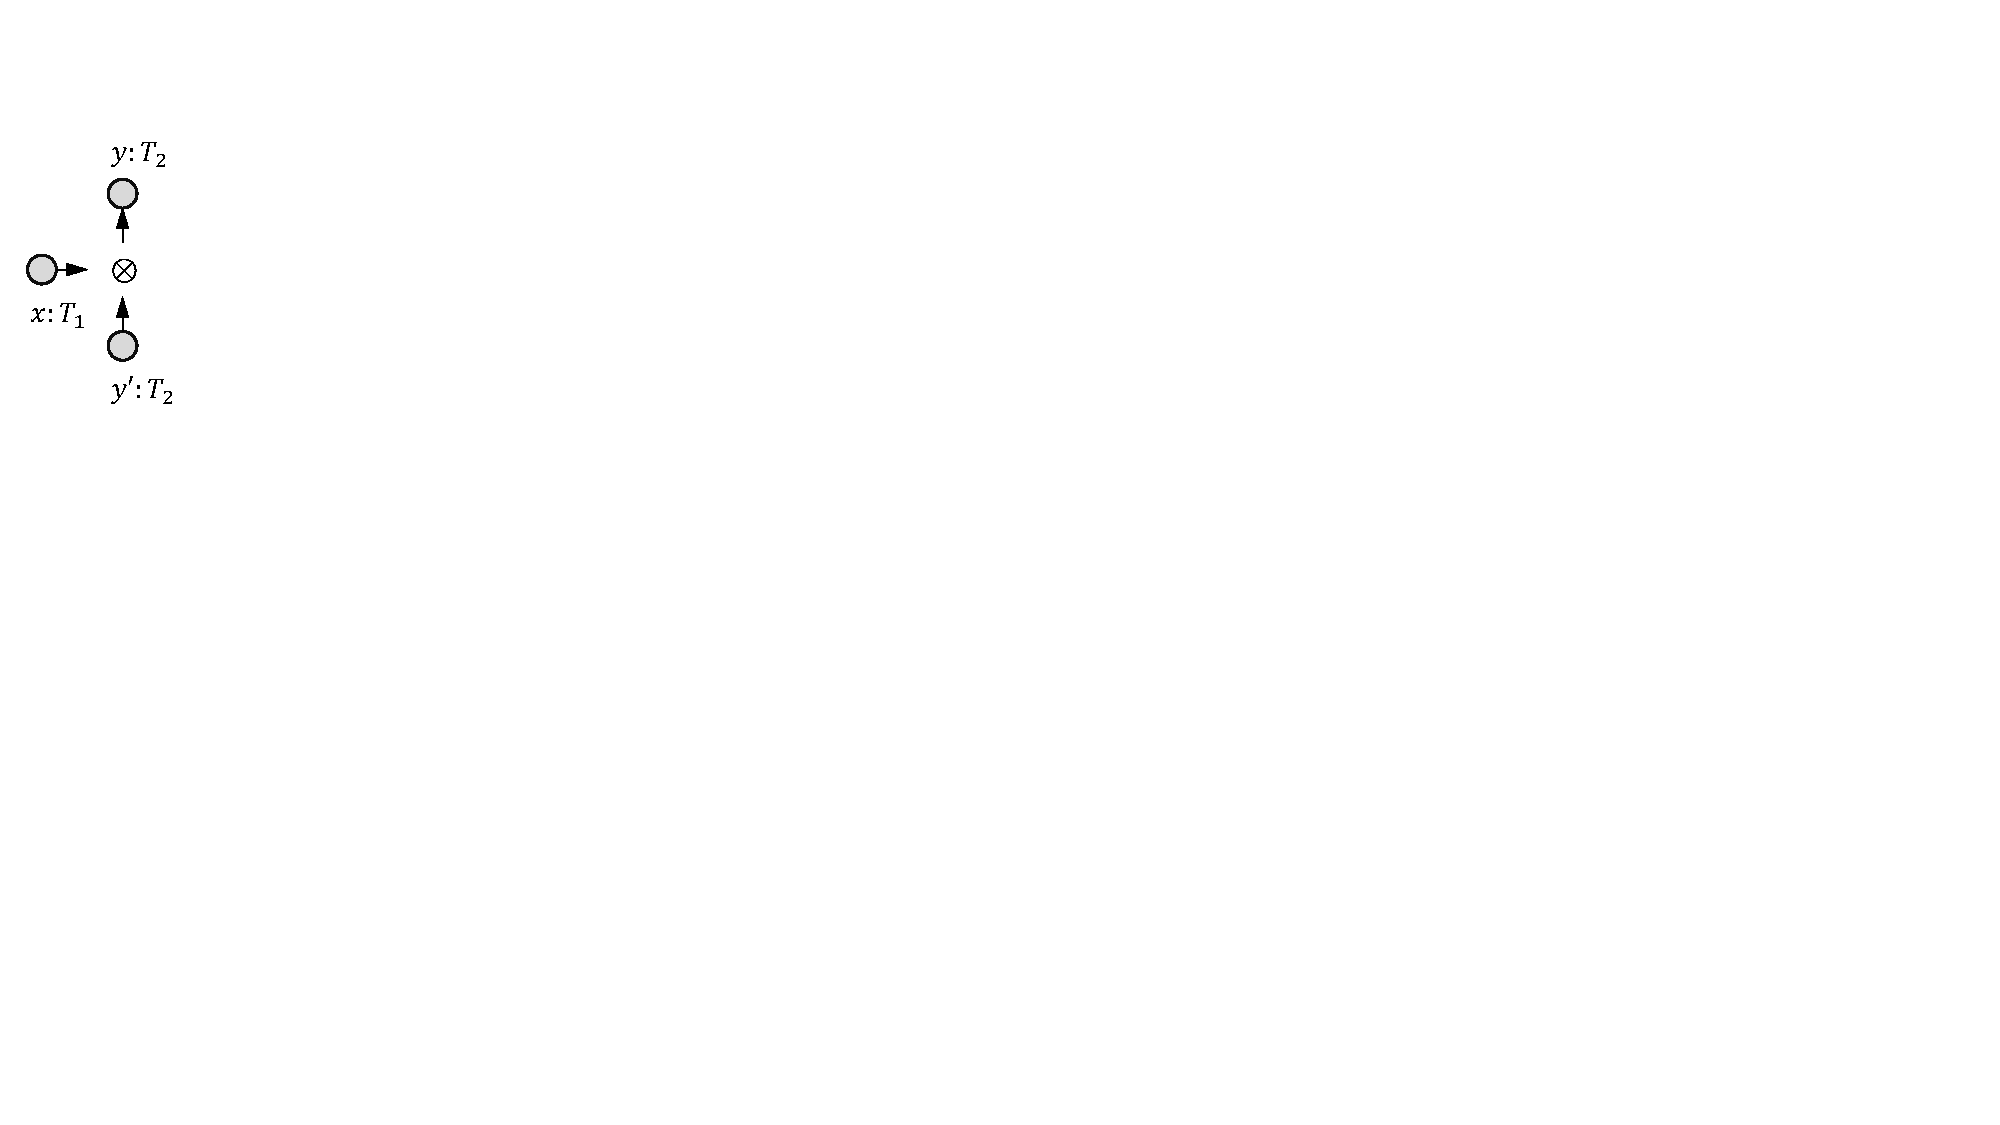
\includegraphics[width=0.1\textwidth]{figures/scan_step.pdf}
%     \caption{A single RNN computation step.}
%     \label{scan-step}
% \end{figure}

% Figure \ref{rnn-layer1} shows an algorithm developer's conceptual model of an RNN layer (the unrolled computational graph in mainstream deep learning frameworks) applied to tokens from a sequence.

% \begin{figure}[h]
%   \centering
%   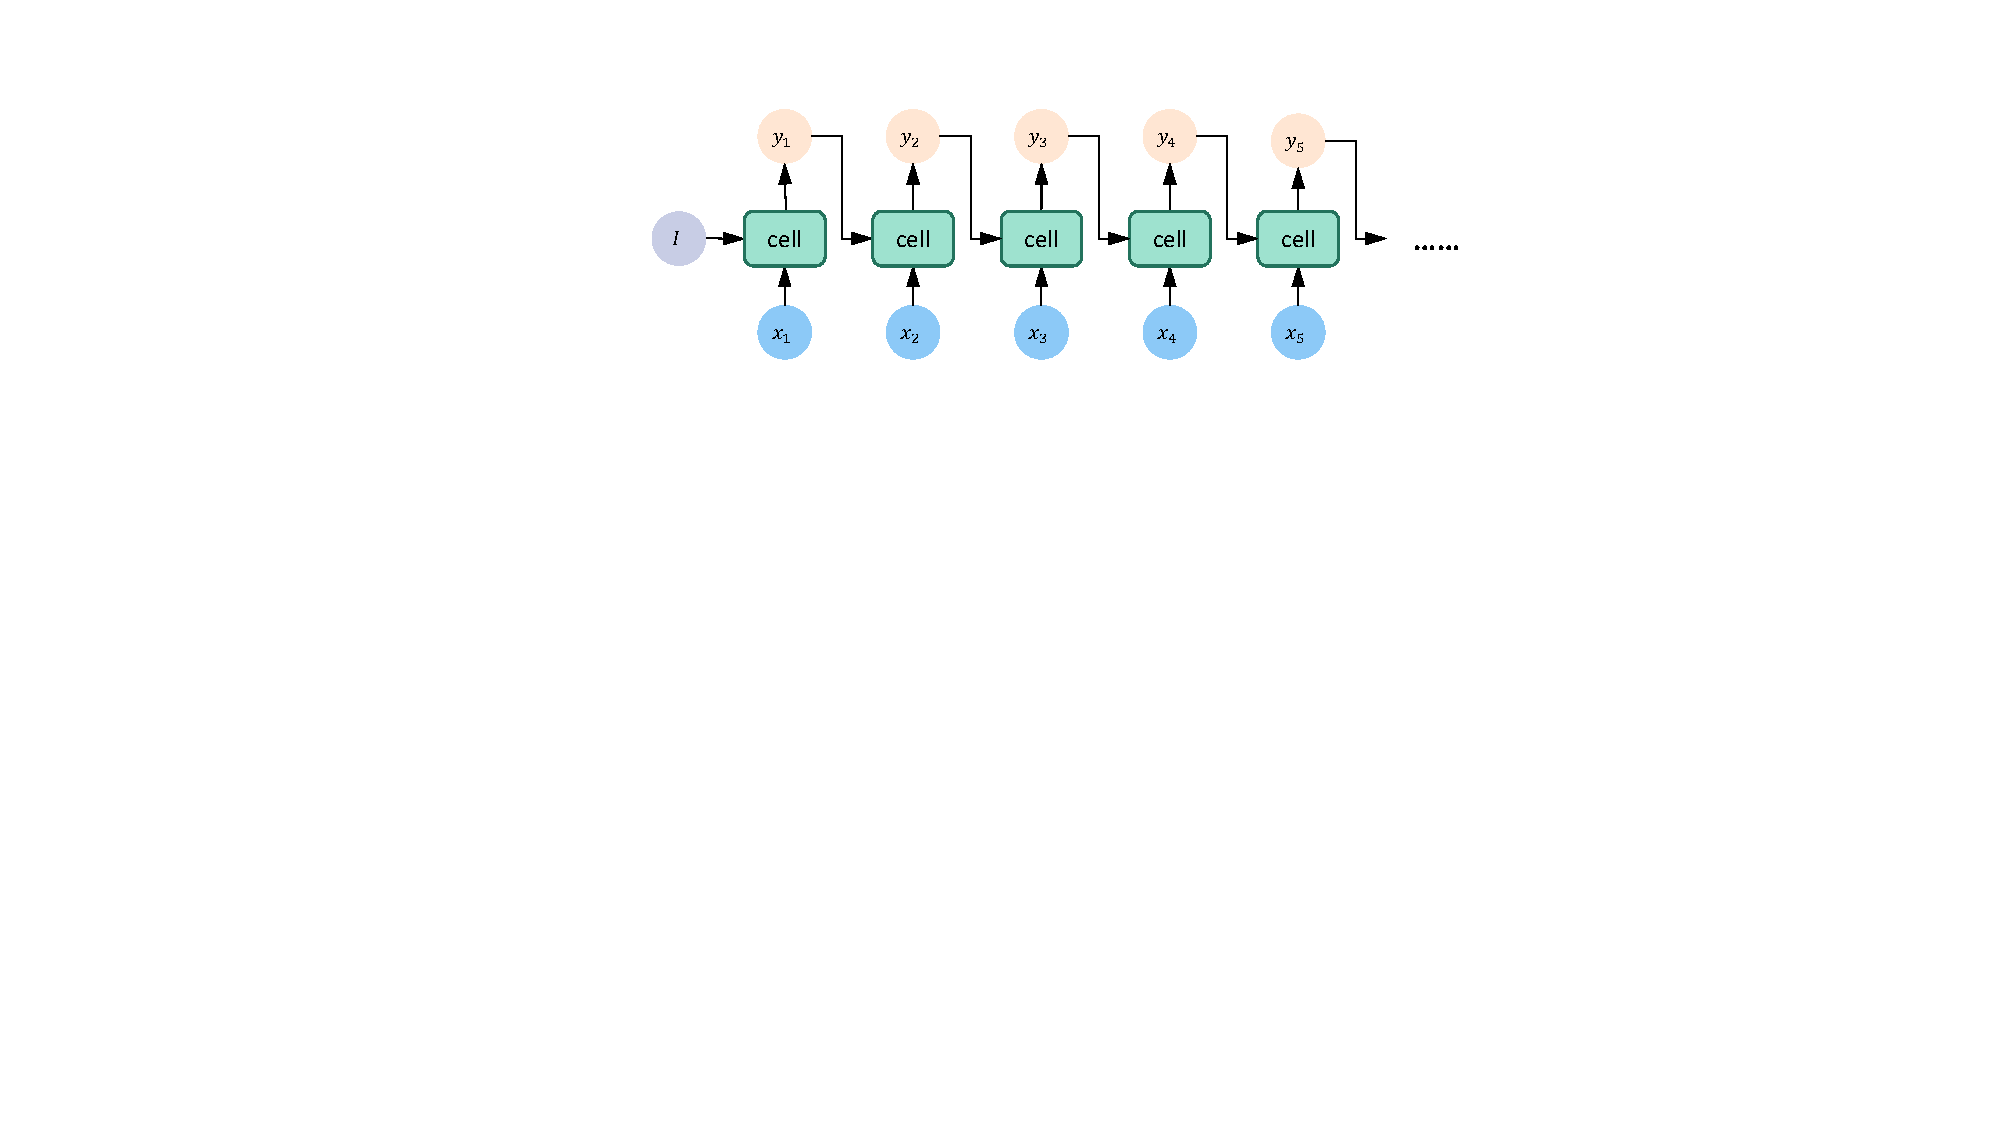
\includegraphics[width=0.5\textwidth]{figures/rnn_layer1.pdf}
%   \caption{An algorithm developer's conceptual model of an RNN layer applied to a single sequence.}
%   \label{rnn-layer1}
% \end{figure}

% An RNN layer is usually trained with a batch of sequences. Figure \ref{rnn-layer2} shows applies an RNN layer to multiple sequences simultaneously and Listing \ref{rnn-layer-code} is the corresponding codes using FractalTensor constructs.

% \begin{figure}[h]
%   \centering
%   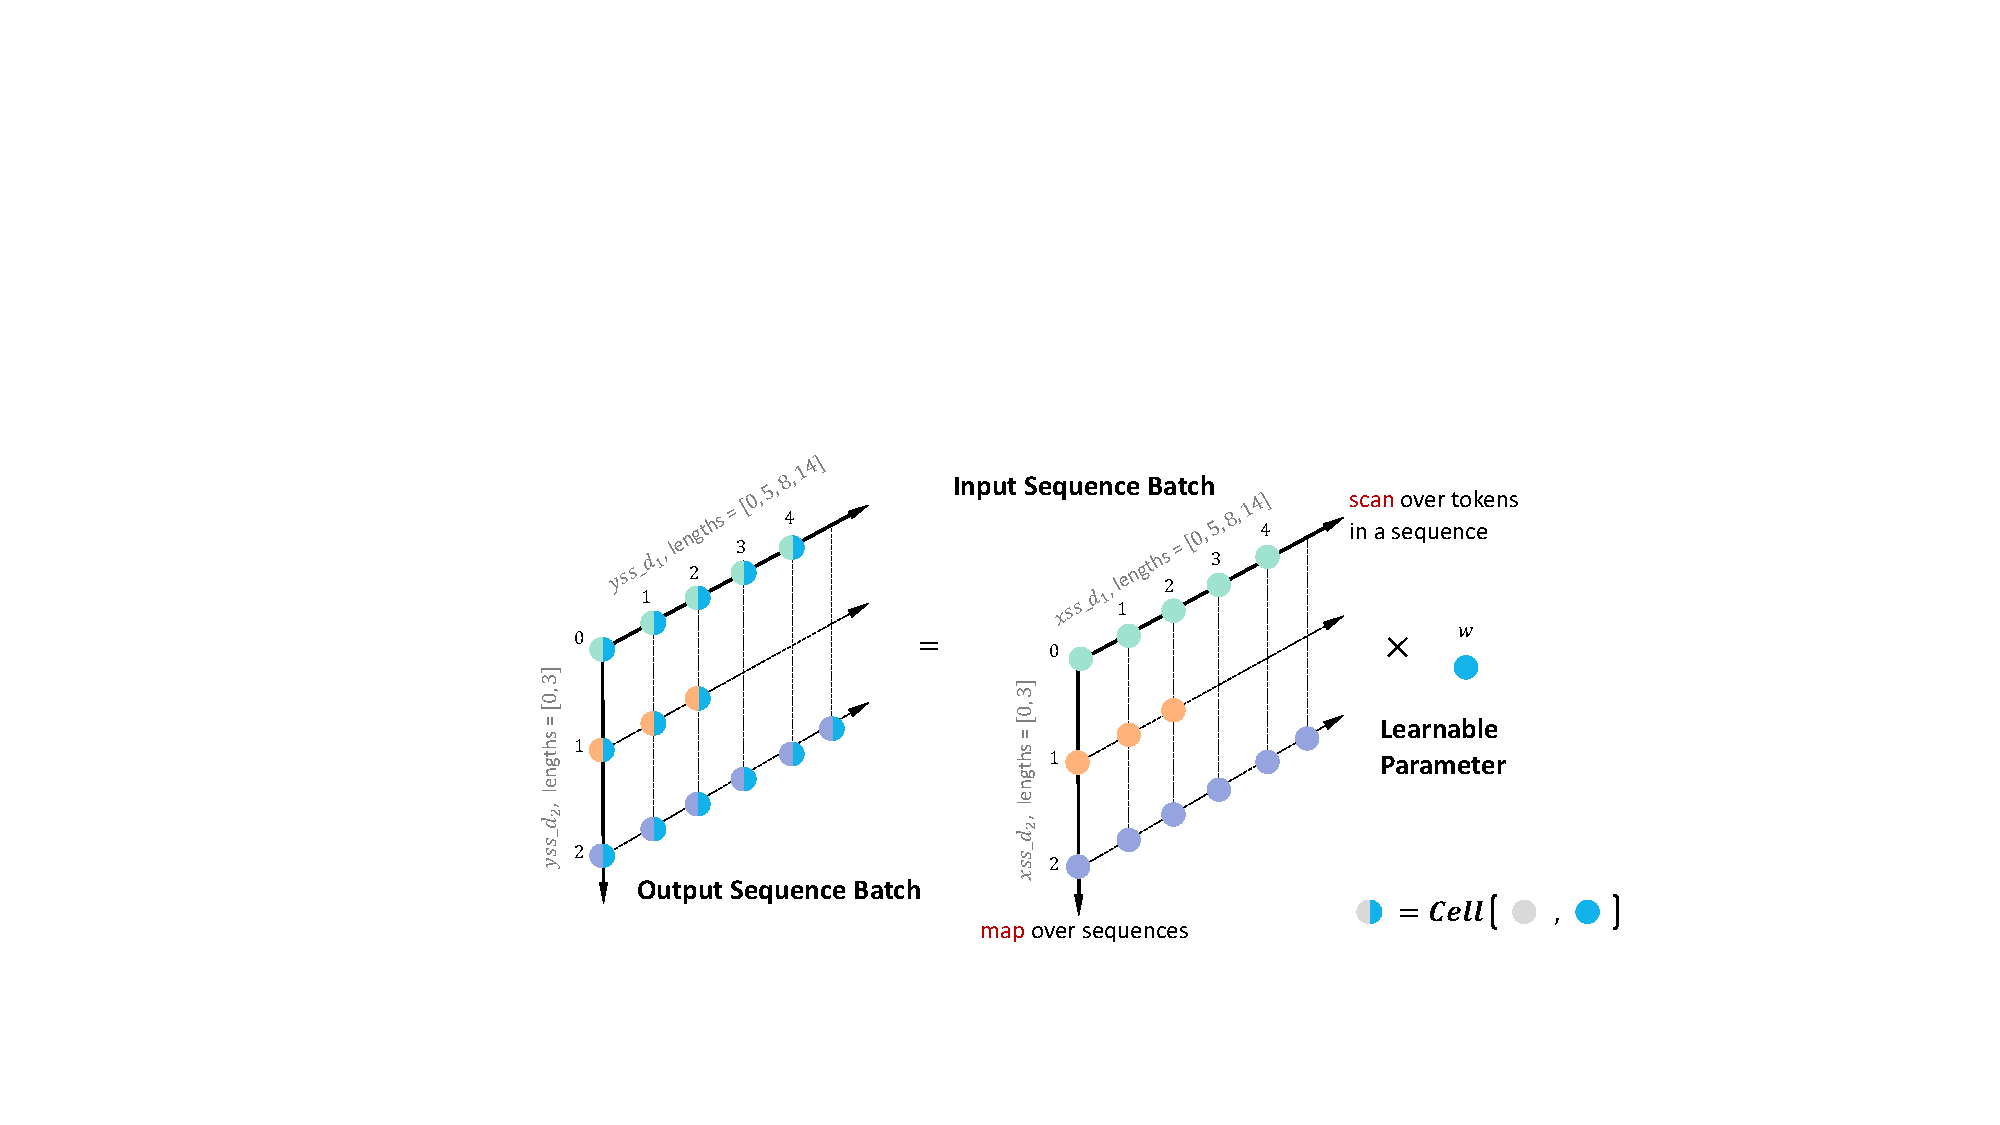
\includegraphics[width=0.6\textwidth]{figures/rnn_layer2.pdf}
%   \caption{An RNN layer applied to multiple sequences.}
%   \label{rnn-layer2}
% \end{figure}

% \lstset{
%   frame=lrtb,
%   backgroundcolor=\color{aliceblue},
%   numbers=left,
%   numbersep=5pt,
%   numbersep=1em,
%   xleftmargin=1em
% }
% \begin{lstlisting}[language=fractaltensor-hello-world, caption={用Parallel Pattern \textcolor{red}{\textit{map}}和\textcolor{red}{\textit{scan}}的嵌套compose 一个RNN layer}, label={rnn-layer-code}]
% xss: [][]float32[1, 512] = ...  // A batch of input sequences
% (:\textbf{\textcolor{dkgreen}{w}}:): float32[512, 512] = ...  // Learnable parameter for the UDF

% // yss: [][]float32[1, 512], the output buffer
% (:\textbf{\textcolor{dkgreen}{yss}}:) = xss.map(xs (:$\Rightarrow$:) {
%     ys = xs.scan(s, x (:$\Rightarrow$:) {
%         y = x @ (:\textbf{\textcolor{dkgreen}{w}}:) + s  // UDF is small math function
%     }, initializer=zeros),
% })
% \end{lstlisting}

% \begin{lstlisting}[language=cplus, caption={Listing \ref{rnn-layer-code}的imperative style 语法等价形}]
% xss: [][]float32[1, 512] = ...  // token batch
% (:\textbf{\textcolor{dkgreen}{w}}:): float32[512, 512] = ... // UDF的可学习参数
% yss: [][]float32[1, 512] = ... // 输出buffer

% L: const int[3] = [5, 3, 6]
% N: int = len(xss)

% for i = [0, N) {  // 对应了全并行的map
%   for j = [0, L[i]) {  // 对应了携带数据流依赖的scan
%     if j == 0:
%       s = zeros
%     else:
%       s = yss[i][j - 1]
%     x = xss[i][j]
    
%     yss[i][j] = x @ w + s
%   }
% }
% \end{lstlisting}


\newpage
\subsection{Stacked RNNs}

\begin{figure}[h]
  \centering
  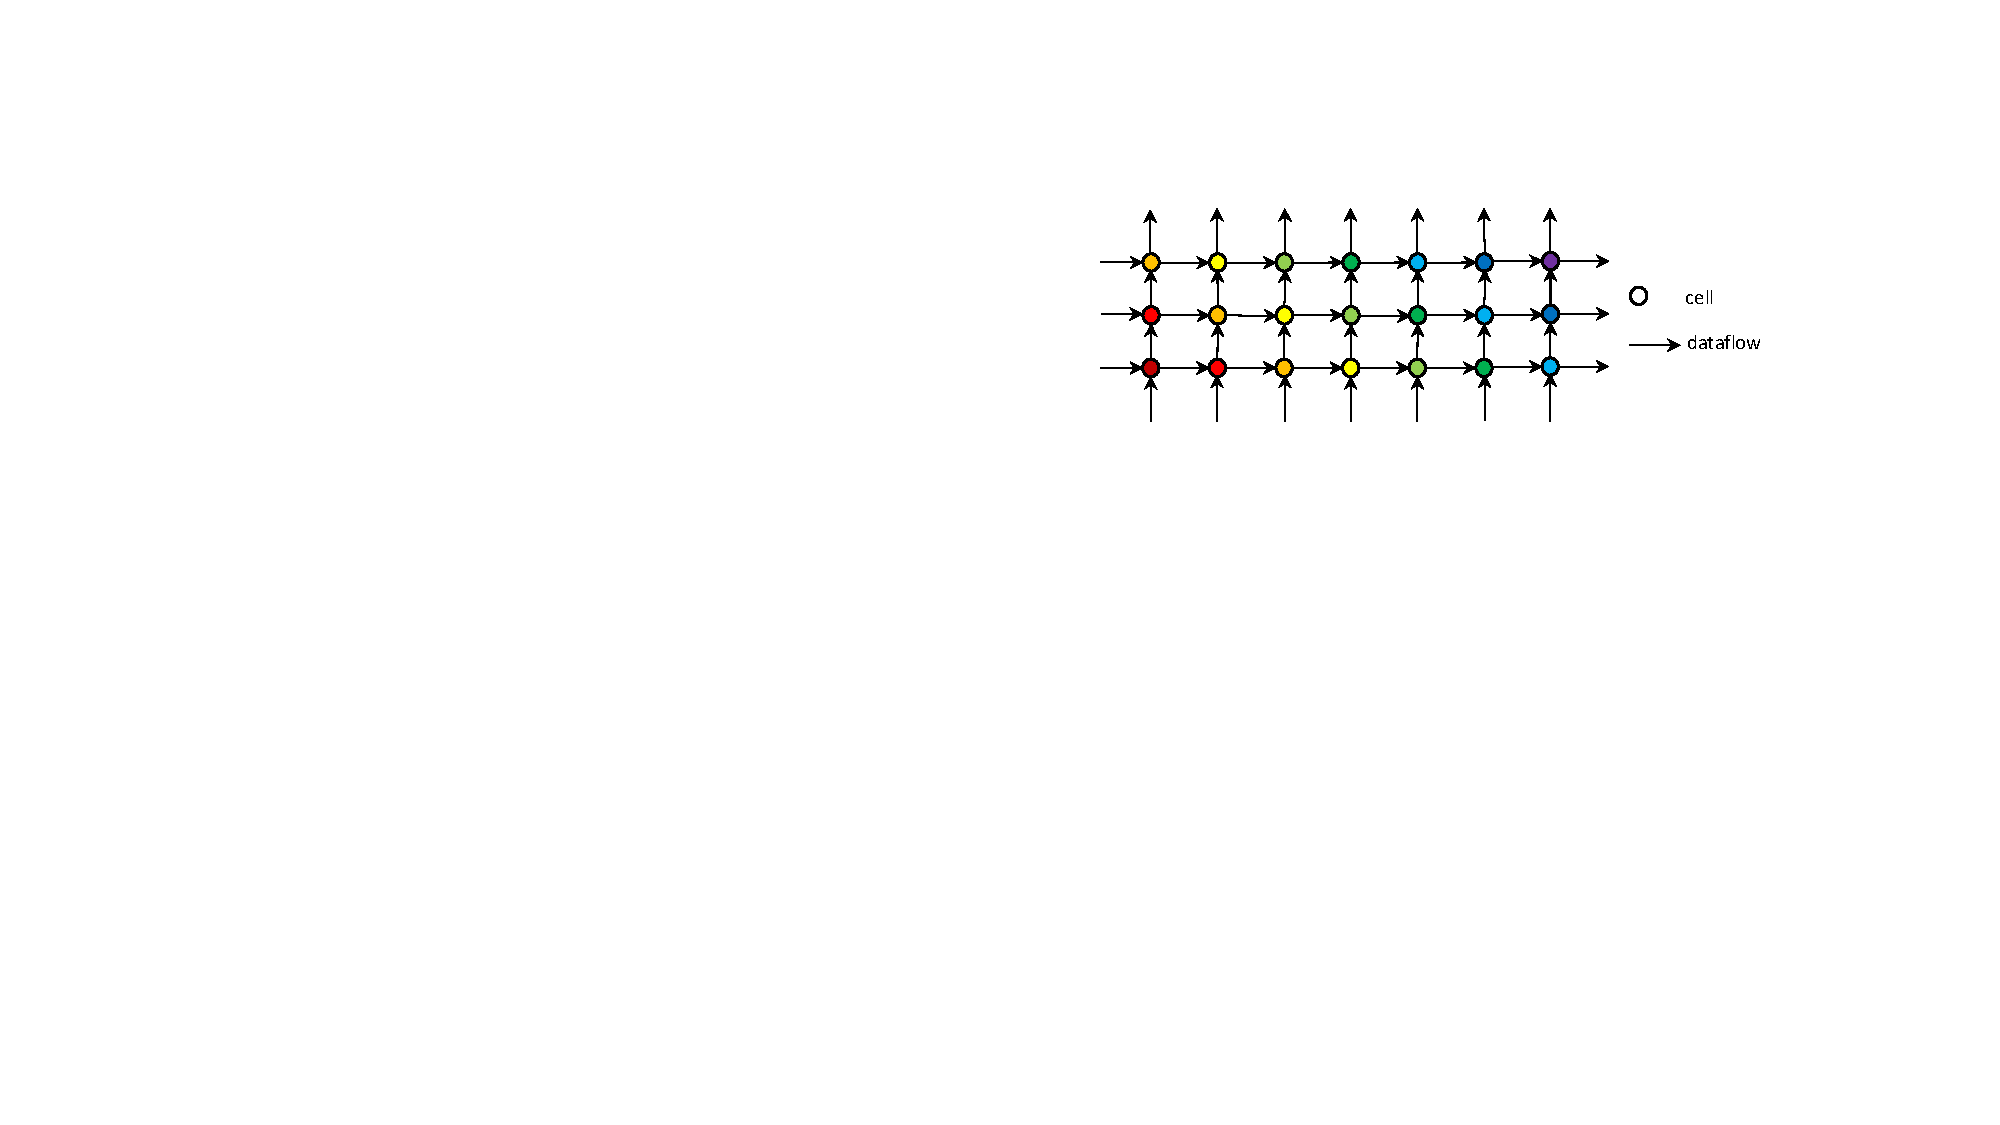
\includegraphics[width=0.6\textwidth]{figures/signal_flow_structure_of_stacked_rnn.pdf}
  \caption{Stacked RNN网络的数据流图}\label{fig:dataflow-stacked-rnn}
\end{figure}

一个optimizing compiler最关心的问题是:检测一个算法天生的\textcolor{blue}{最大并行性}和\textcolor{blue}{最大数据复用机会}。如果能检测到就有可能通过调度策略的设计,在一个并行后端上达到高效执行。
我们无论用什么样的语法形式去写RNN网络,对optimizing compiler检测和利用并行性最重要的是抽取出图\ref{fig:dataflow-stacked-rnn}这样的一个数据流图结构。
\vspace{1em}

\begin{lstlisting}[language=fractaltensor-hello-world, caption={用parallel pattern compose stacked RNN网络}, label={stacked-rnn-code1}]
xss: [][]float32[1, 512] = ...  // A batch of input sequences
ws: [3]float32[512, 512] = ...  // UDF的可学习参数

ysss = xss.map(xs => {  // ysss: [[[float32[1, 512]]]]
  yss = ws.scan(ss, w => {  // scan over depth
    ys = ss.scan(s, x => {  // scan over sequence length
      y = x @ w + s  // the user-defined cell function.
    }, initializer=zeros),
  }, initializer=xs),
})
\end{lstlisting}

\begin{lstlisting}[language=fractaltensor-hello-world, caption={Listing \ref{stacked-rnn-code1} 的另一种语法等价形}, label={stacked-rnn-code}]
xss: [][]float32[1, 512] = ...  // A batch of input sequences
ws: [3]float32[512, 512]] = ...  // UDF的可学习参数

ysss = xss.map(xs => {  // ysss: [][][]float32[1, 512]
  yss = xs.scan(ss, x => {  // scan over sequence length
    ys = zip(ss, ws).scan(s0, s, w => { // scan over depth
      y = s0 @ w + s  // UDF是一个非常小的纯线性代数公式
    }, initializer=x),
  }, initializer=repeat(zeros, ws.length)),
})
\end{lstlisting}

这里有一个非常漂亮的特性,对并行性检测和利用至关重要,\textit{\textbf{\textcolor{red}{用map,reduce,scan 这样的SOAC写出来的嵌套循环程序,一定是一个可任意换序的循环嵌套}}}。

\newpage
\begin{lstlisting}[language=cplus, caption={Stacked RNN的imperative style语法等价形,这里把UDF替换成LSTM的cell function}, label={stacked-lstm-imperative}]
for i in range(N):  // corresponds to map
  for j in range(D):  // corresponds to fold
    for k in range(L):  // corresponds to scan
      if j == 0 and k == 0: // control region S0
        h_prev = zeros
        c_prev = zeros
        x = xss[i][k]
      elif j == 0 and k > 0: // control region S1
        h_prev = hsss[i][j][k - 1]
        c_prev = csss[i][j][k - 1]
        x = xss[i][k]
      elif j > 0 and k == 0: // control region S2
        h_prev = zeros
        c_prev = zeros
        x = hsss[i][j - 1][k]
      else:  // control region S3
        h_prev = output[i][j][k - 1]
        c_prev = output[i][j][k - 1]
        x = hsss[i][j - 1][k]
  
      h, c = lstm_cells[j](x, h_prev, c_prev) // the UDF
      hsss[i][j][k] = h
      csss[i][j][k] = c
\end{lstlisting}

Listing \ref{stacked-lstm-imperative} 是stacked RNN网络的语法等价形式,唯一变化是这里我们把UDF替换成LSTM cell:
$c_t, h_t = \textbf{lstm\_cell}\left(\vec{x}_t,\vec{h}_{t-1}, \mathbf{Params} \right)$,具体是由下面六个线性代数公式定义:

\begin{align}
     f_t &= \sigma_g\left(\mathbf{W}_f\vec{x}_t + \mathbf{U}_f \vec{h}_{t-1}+\vec{b}_f\right) \\
     i_t &= \sigma_g\left(\mathbf{W}_i\vec{x}_t + \mathbf{U}_i \vec{h}_{t-1}+\vec{b}_i\right) \\
     o_t &= \sigma_g\left(\mathbf{W}_o\vec{x}_t + \mathbf{U}_o \vec{h}_{t-1}+\vec{b}_o\right) \\
     \widetilde{c}_t &= \sigma_c\left(\mathbf{W}_c\vec{x}_t + \mathbf{U}_c \vec{h}_{t-1}+\vec{b}_c\right) \\
     c_t &= f_t \odot c_{t-1} + i_t \odot \widetilde{c}_t \\
     h_t & = o_t \odot \sigma_h\left(c_t\right)
\end{align}

于是,我们会面对这样一个问题:\textit{\textbf{\textcolor{tomato}{给定了这样一组嵌套在loop nest之中的线性代数公式:LSTM cell,是否有办法让一个optimzing compiler基于程序中的general facts,同时给定硬件参数,自动推断出一个好的并行实现方案?}}} (我们的思考甚至\textit{可以安全地忽略}这个loop nest到底是用哪一种语法形式写出来的)。

\begin{figure}[h]
  \centering
  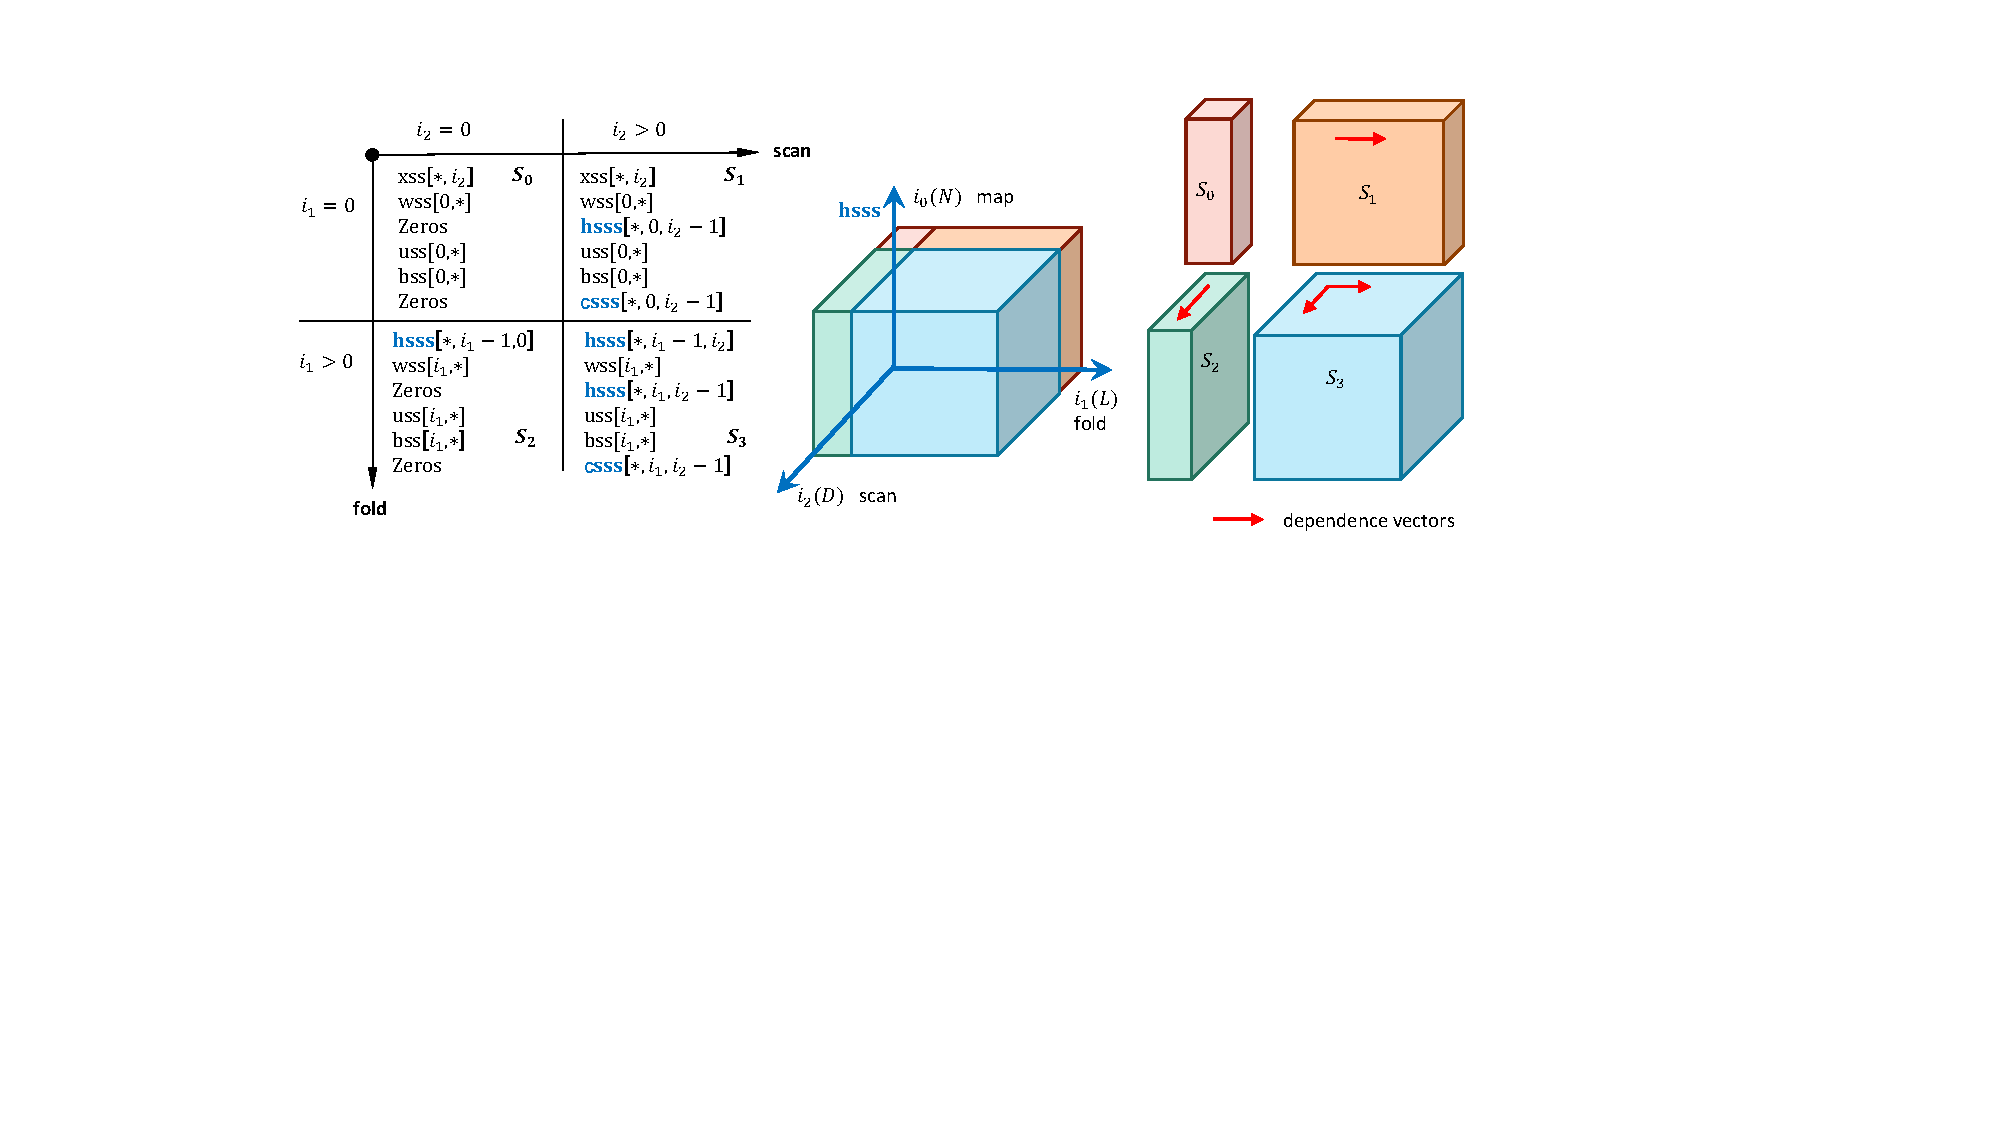
\includegraphics[width=1.\textwidth]{figures/cond_branchs.pdf}
  \caption{编译stacked RNNs计算的复杂性}\label{cond_branchs}
\end{figure}